% This is samplepaper.tex, a sample chapter demonstrating the
% LLNCS macro package for Springer Computer Science proceedings;
% Version 2.21 of 2022/01/12
%
\documentclass[runningheads]{llncs}
%
\usepackage[T1]{fontenc}
% T1 fonts will be used to generate the final print and online PDFs,
% so please use T1 fonts in your manuscript whenever possible.
% Other font encondings may result in incorrect characters.
%
\usepackage{graphicx}
% Used for displaying a sample figure. If possible, figure files should
% be included in EPS format.
%
% If you use the hyperref package, please uncomment the following two lines
% to display URLs in blue roman font according to Springer's eBook style:
%\usepackage{color}
%\renewcommand\UrlFont{\color{blue}\rmfamily}
%
\usepackage[backend=biber]{biblatex}
\bibliography{../../AGI-book}

\usepackage{amsmath}
\usepackage{amssymb}
\usepackage{float}
\usepackage[many]{tcolorbox}

\newcommand{\circled}[1]{{\textcircled{\sffamily \scriptsize{#1}}}}
\tcbset{on line, 
	boxsep=3pt, left=0pt,right=0pt,top=0pt,bottom=0pt,
	colframe=red,colback=pink,
	highlight math style={enhanced}
}
\newcommand{\atom}{\vcenter{\hbox{\tcbox{\mbox{     }}}}}

%\usepackage[nodisplayskipstretch]{setspace}
%\setstretch{0.7}

%\setlength{\belowdisplayskip}{0pt} \setlength{\belowdisplayshortskip}{0pt}
%\setlength{\abovedisplayskip}{0pt} \setlength{\abovedisplayshortskip}{0pt}

%\setlength{\abovedisplayskip}{10pt}
%\setlength{\belowdisplayskip}{10pt}

\begin{document}
%
\title{Transformer as Symbolic Logic Rule-Base}
%
%\titlerunning{Abbreviated paper title}
% If the paper title is too long for the running head, you can set
% an abbreviated paper title here
%
\author{King Yin Yan\inst{1}\orcidID{0009-0007-8238-2442} \and
Ziyu Zhou\inst{2}}
%
\authorrunning{Yan et al.}
% First names are abbreviated in the running head.
% If there are more than two authors, 'et al.' is used.
%
\institute{
	\email{general.intelligence, subfishzhou @gmail.com} \and
	Beijing University of Posts and Telecommunications
}
%
\maketitle              % typeset the header of the contribution
%
\begin{abstract}
This short paper shows that Transformers \cite{Vaswani2017} can implement a certain flavor of symbolic-logic rules engine.  As Transformers are shown to be Turing universal\cite{Perez2021}, this should come as no surprise, but such an insight could be a cornerstone for neuro-symbolic AGI.

\keywords{Transformer \and Self-Attention \and symbolic logic \and neuro-symbolic AI}
\end{abstract}
%
%

Fig. \ref{Self-Attention} shows a schematic diagram of Transformer Self-Attention, assuming the reader is familiar with its workings.
\begin{figure}[H]
	\centering
	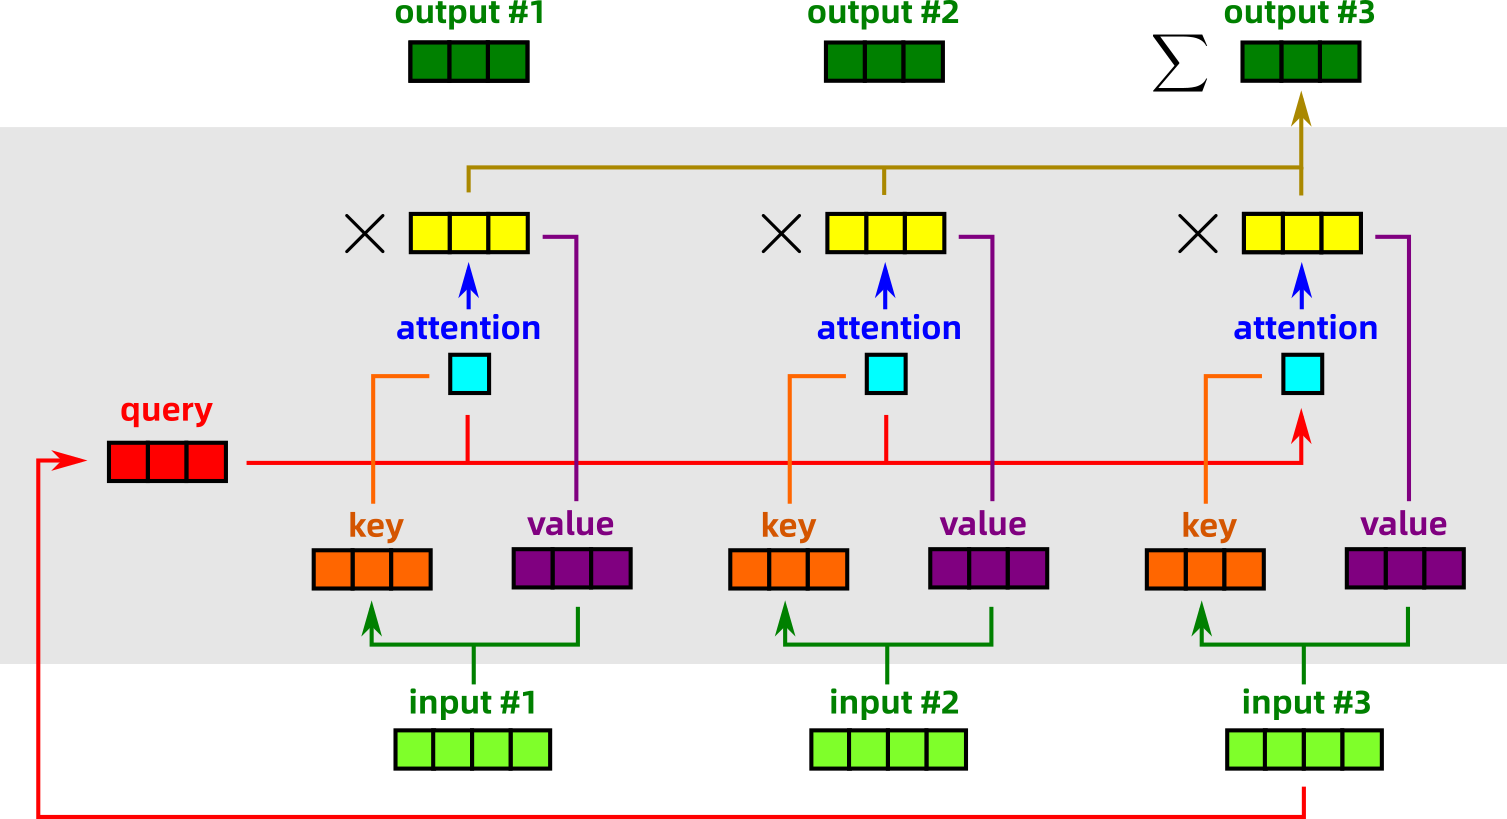
\includegraphics[scale=0.6]{Self-Attention.png}
	\caption{Schematic of the Transformer Self-Attention}
	\label{Self-Attention}
\end{figure}

``Input'' tokens are translated to $Q,K,V$ (query, key, value)'s via matrix multiplication, which can be regarded as a kind of table look-up, or \textbf{memory store} (Fig. \ref{Abstract-Self-Attention}\circled{A}).  From an abstract point of view, the Transformer has the structure of Fig. \ref{Abstract-Self-Attention}\circled{B}, which gives rise to its \textbf{equivariance} property (if input elements are swapped in a certain order, the output elements changes the same way).
\begin{figure}[H]
	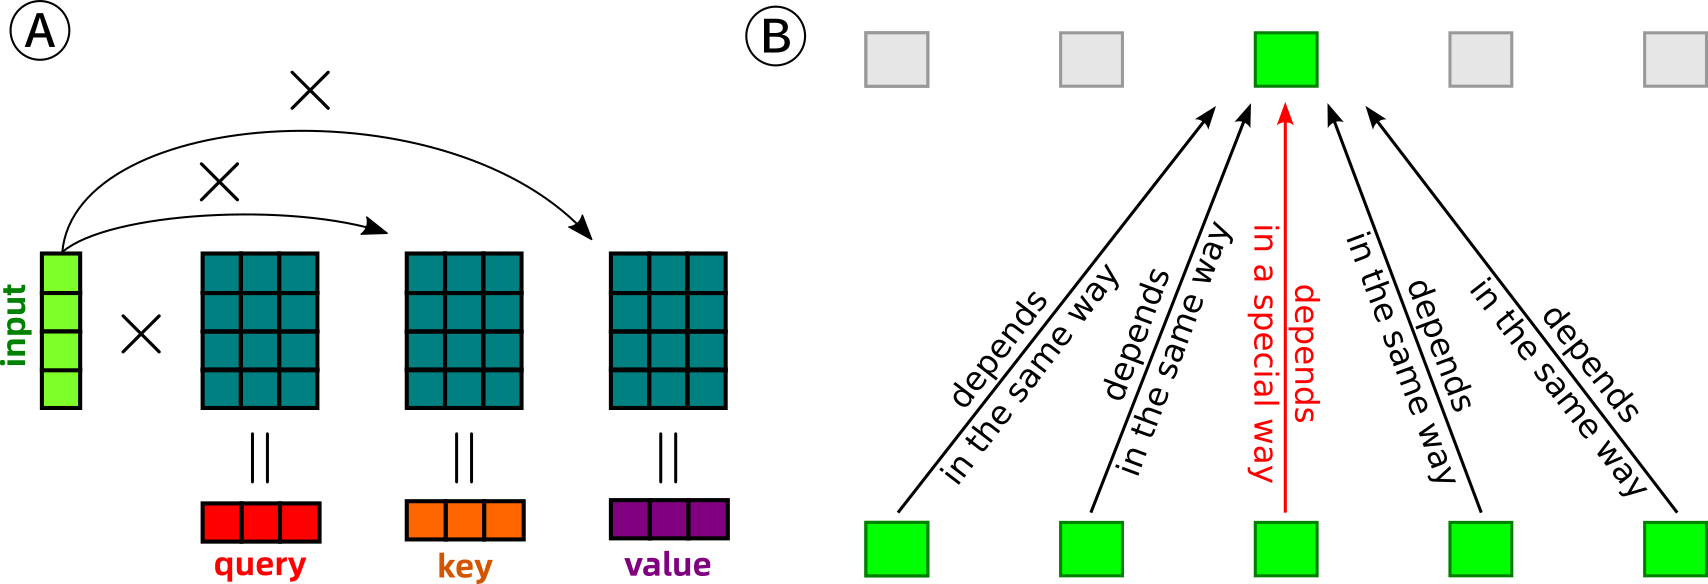
\includegraphics[scale=0.55]{Abstract-Self-Attention.png}
	\caption{\circled{A}: $Q,K,V$ as lookup tables. \circled{B}: abstract self-attention}
	\label{Abstract-Self-Attention}
\end{figure}

The equivariance property corresponds to the \textbf{exchangeability} of logic propositions:
\begin{equation}
A \wedge B \quad \Leftrightarrow \quad B \wedge A
\end{equation}
For example:
\begin{equation}
\mbox{it's raining} \wedge \mbox{I'm heart-broken} \quad \Leftrightarrow \quad \mbox{I'm heart-broken} \wedge \mbox{it's raining}
\end{equation}
Propositions are made up of \textbf{atomic concepts}, but at this sub-propositional level, atoms cannot be permuted freely, eg:
\begin{equation}
\mbox{I} \cdot \mbox{love} \cdot \mbox{her} \quad \neq \quad \mbox{she} \cdot \mbox{loves} \cdot \mbox{me}
\end{equation}
otherwise there would be no such things as heart-breaks.

Now recall some basic notions of \textbf{classical logic-based AI}.  Its basic architecture is as in Fig. \ref{LBAI}.
\begin{figure}[H]
	\centering
	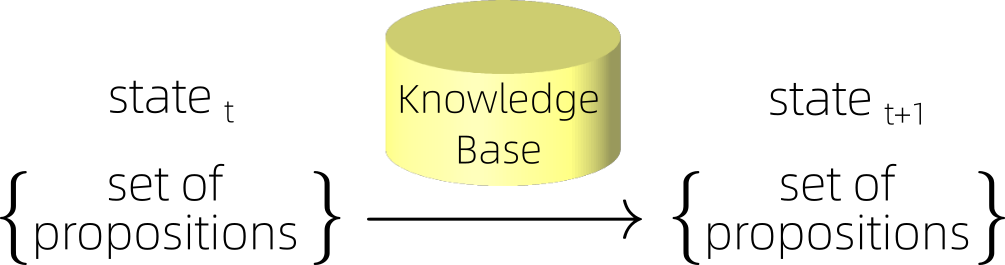
\includegraphics[scale=0.6]{LBAI.png}
	\caption{Basic architecture of classical logic-based AI}
	\label{LBAI}
\end{figure}

There would be a huge number of rules in the Knowledge Base, and the system needs to match these rules one by one against propositions in the system's \textbf{state} (= working memory) (Fig. \ref{rules-matching.png}).
\begin{figure}[H]
	\centering
	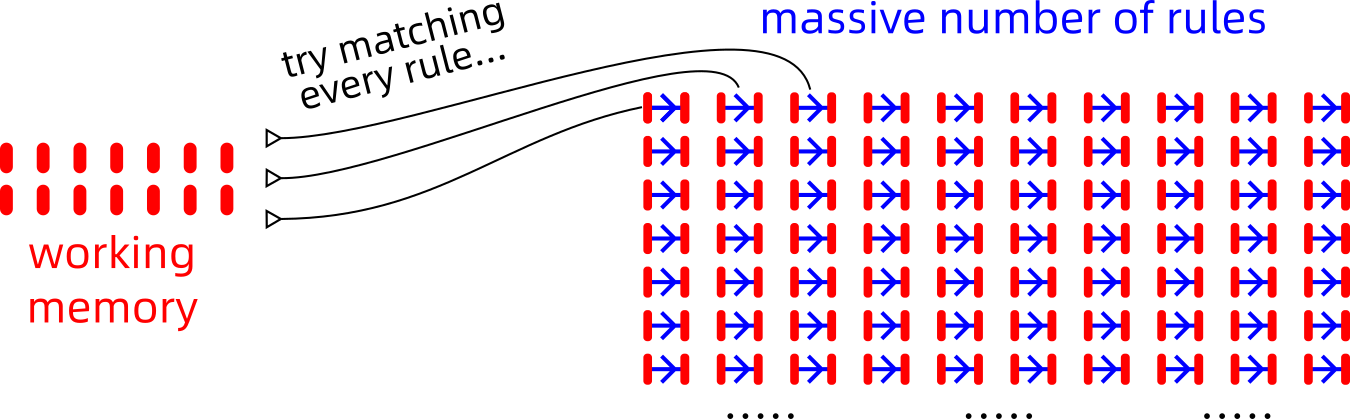
\includegraphics[scale=0.5]{rules-matching.png}
	\caption{Vastness of rules matching}
	\label{rules-matching.png}
\end{figure}

For the Transformer, it is a kind of memory stored \textbf{between} input elements (stored as the $Q, K, V$ matrices), and it \textbf{implicitly} plays the role of a logic rule-base (Fig. \ref{Attention-as-Rete}).  This is similar to message-passing in a graph.
\begin{figure}[H]
	\centering
	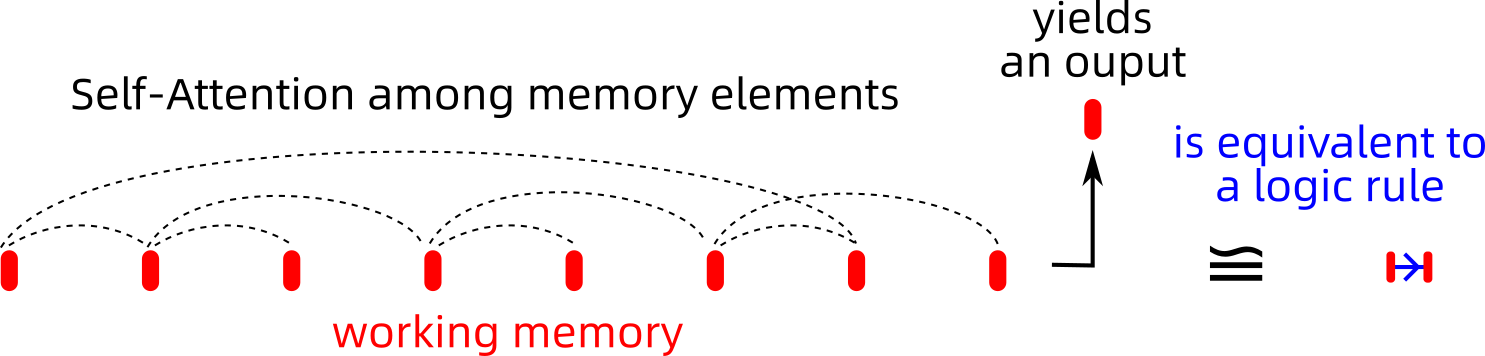
\includegraphics[scale=0.5]{Attention-as-Rete.png}
	\caption{Self-Attention as a kind of rules-matching mechanism}
	\label{Attention-as-Rete}
\end{figure}

A crucial insight is that the \textbf{Self-Attention} mechanism had its origin in NTMs (\textbf{Neural Turing Machines}) \cite{Graves2014}.  The Turing machine needs to have a ``memory tape'' but in the neural setting this memory must be \textit{differentiable}.  If the memory is addressed by an index $i \in \mathbb{N}$, then it won't be differentiable.  So they came up with a \textbf{content-addressable} memory mechanism where a memory matrix is looked up using the ``query-key-value'' method.  A nice explantion of NTMs can be found in the book \textit{Fundamentals of Deep Learning} \cite{Buduma2017}.

Now consider LLMs (\textbf{Large Language Models}) such as BERT or GPT.  Given a natural-language sentence, we'd like to convert or \textbf{decompose} it into a list of logic propositions (Fig. \ref{Transformer-layer1}).
\begin{figure}[h]
	\centering
	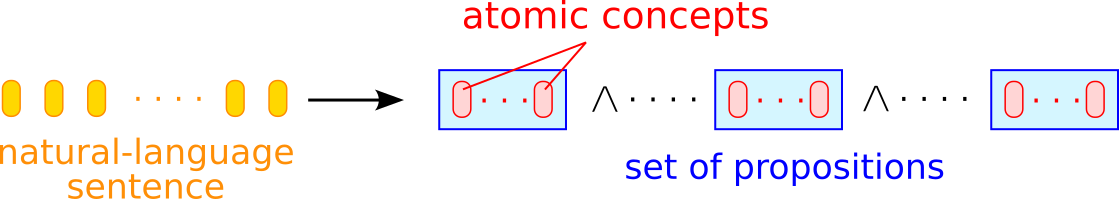
\includegraphics[scale=0.6]{Transformer-layer1.png}
	\caption{}
	\label{Transformer-layer1}
\end{figure}
The structure on the right of Fig. \ref{Transformer-layer1} is the \textbf{mental state} of a logical AI system.  It is composed of (exchangeable) propositions, which are in turn made up of atomic concepts.  This 2-level structure is characteristic of all \textbf{logical} systems.  Surprisingly, I found that the Transformer completely satisfies this 2-level logic structure.

On the \textbf{first layer}, a Transformer transforms each input word token into one proposition (Fig. \ref{Transformer-layers}\circled{A}).
\begin{figure}
	\centering
	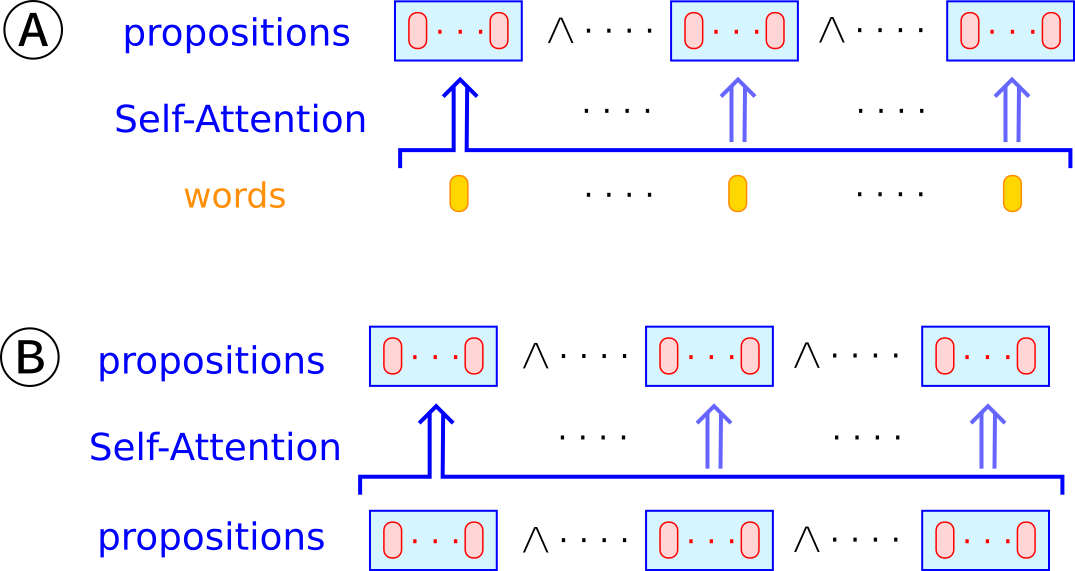
\includegraphics[scale=0.6]{Transformer-layers.png}
	\caption{}
	\label{Transformer-layers}
\end{figure}
The crucial point here is that the propositions are composed of atoms ($\atom$), this can be achieved in the Transformer by vector \textbf{addition}, ie, \textbf{superposition} of atomic concepts.  Note also that the Transformer is equivariant, so we must add ``positional encoding'' to each word, to indicate their ordering.

At \textbf{higher layers}, there is no need for positional encoding, and logic propositions can be freely exchanged, exactly as what happens in Transformers (Fig. \ref{Transformer-layers}\circled{B}).

Note that in the above, every $\Uparrow$ arrow uses the same $(Q,K,V)$ matrices as ``rule-base'', that may limit the number of rules that can be represented.  To circumvent this, \textbf{Multi-Head Attention} allows to use different $(Q,K,V)$ matrices on the same layer.

%
% the environments 'definition', 'lemma', 'proposition', 'corollary',
% 'remark', and 'example' are defined in the LLNCS documentclass as well.
%

% \subsubsection{Acknowledgements} Please place your acknowledgments at
% the end of the paper, preceded by an unnumbered run-in heading (i.e.
% 3rd-level heading).

%
% ---- Bibliography ----
%
% BibTeX users should specify bibliography style 'splncs04'.
% References will then be sorted and formatted in the correct style.
%
% \bibliographystyle{splncs04}
% \bibliography{mybibliography}
%
%\begin{thebibliography}{8}
\printbibliography
\end{document}
